\documentclass[tikz,border=8pt]{standalone}
\usepackage{tikz}
\usetikzlibrary{positioning,arrows.meta,fit,backgrounds,calc}

\begin{document}
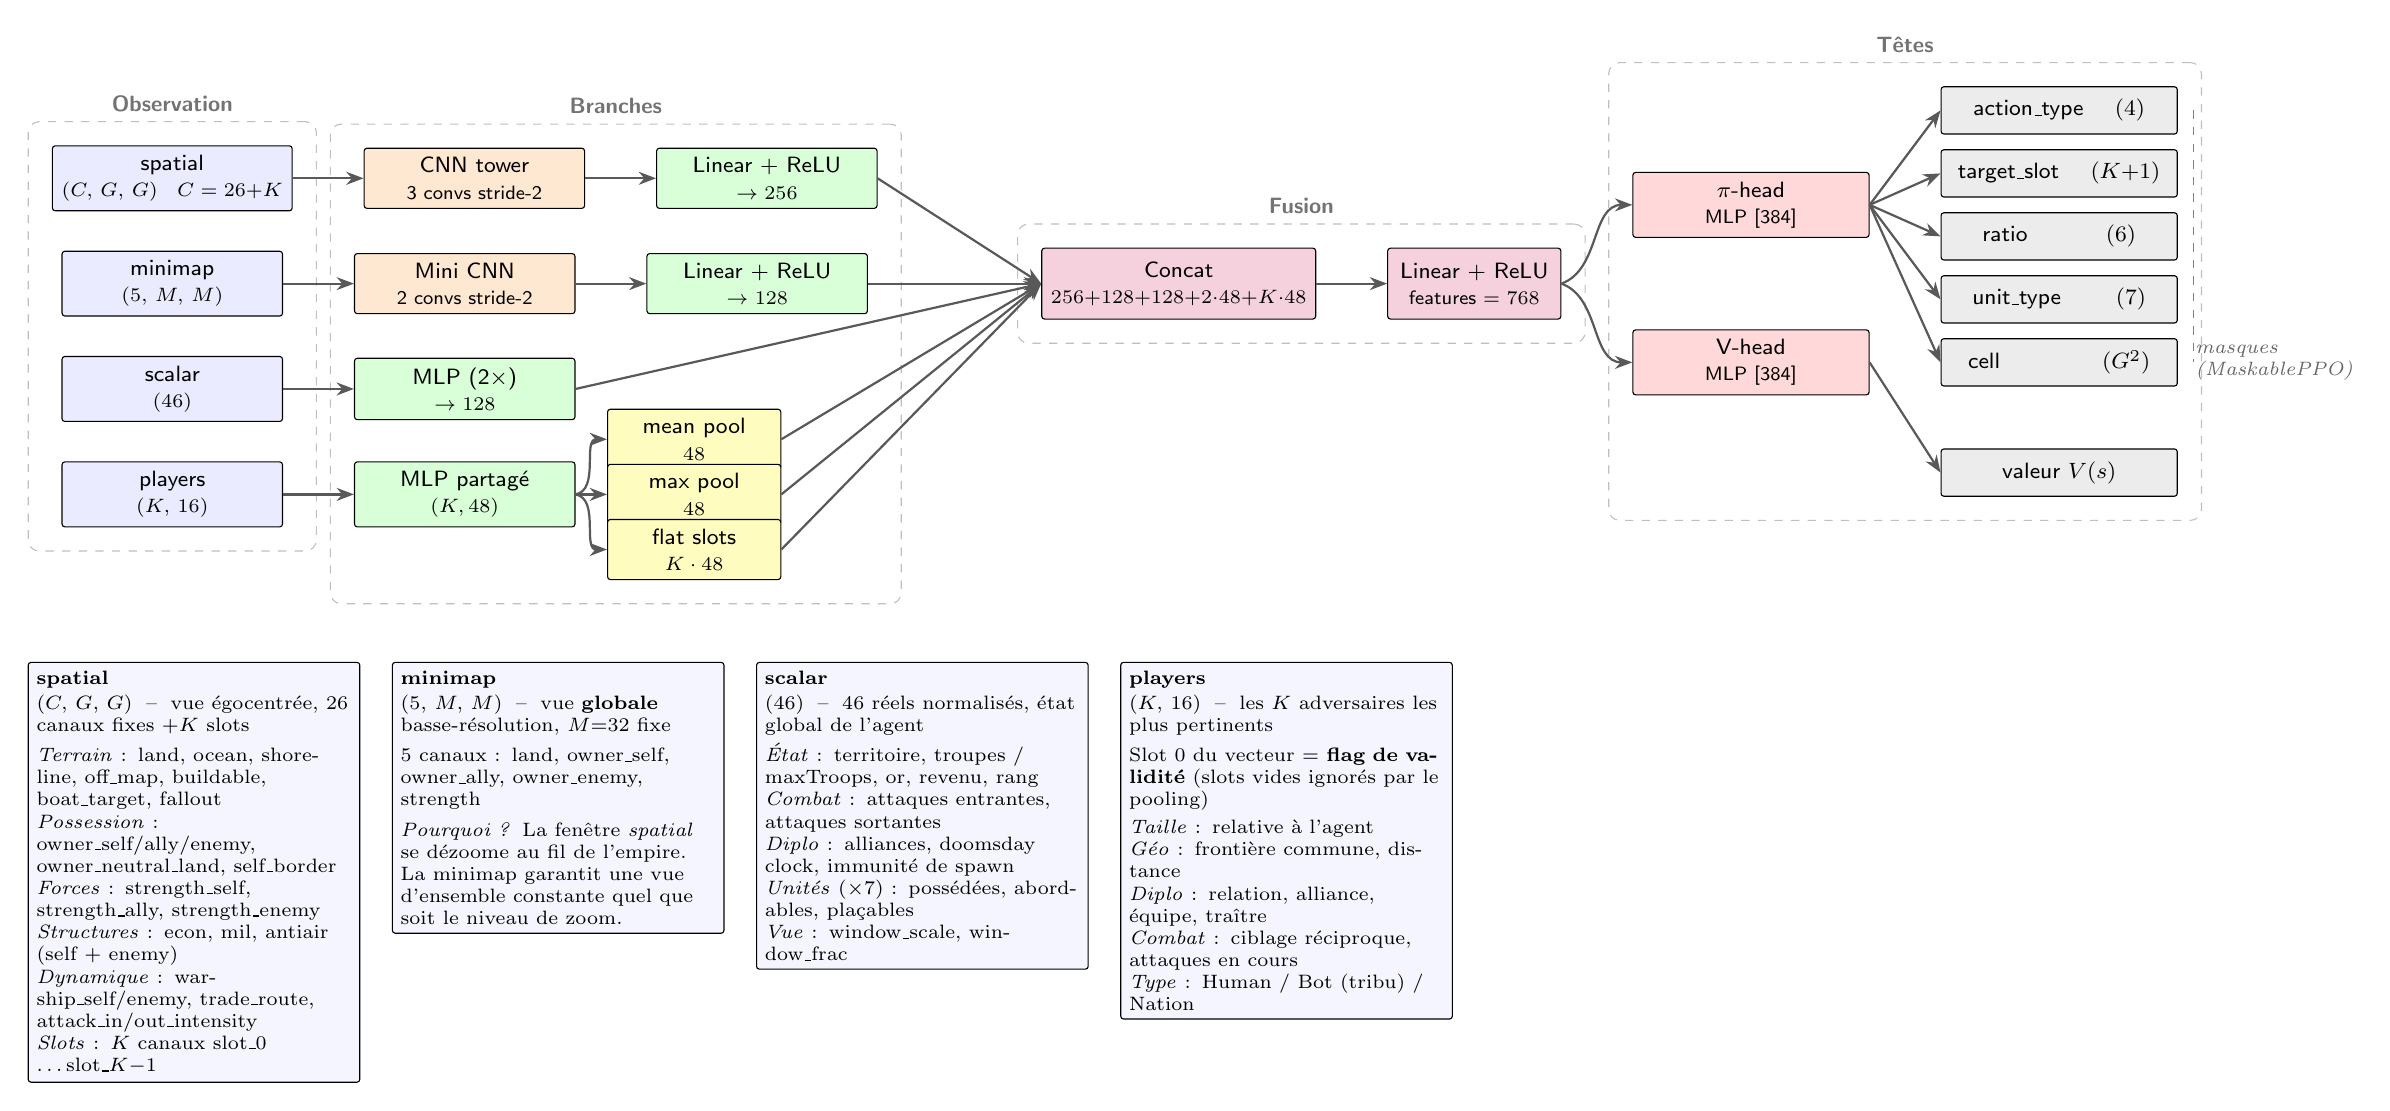
\begin{tikzpicture}[
  font=\sffamily\footnotesize,
  >={Stealth[length=2.2mm]},
  node distance=5mm and 9mm,
  input/.style   ={draw, rounded corners=1pt, fill=blue!8,   minimum width=28mm, minimum height=7mm, align=center},
  cnn/.style     ={draw, rounded corners=1pt, fill=orange!18, minimum width=28mm, minimum height=7mm, align=center},
  mlp/.style     ={draw, rounded corners=1pt, fill=green!15,  minimum width=28mm, minimum height=7mm, align=center},
  pool/.style    ={draw, rounded corners=1pt, fill=yellow!25, minimum width=22mm, minimum height=6mm, align=center},
  fuse/.style    ={draw, rounded corners=1pt, fill=purple!18, minimum width=22mm, minimum height=9mm, align=center},
  head/.style    ={draw, rounded corners=1pt, fill=red!15,    minimum width=30mm, minimum height=7mm, align=center},
  outbox/.style  ={draw, rounded corners=1pt, fill=gray!15,   minimum width=30mm, minimum height=6mm, align=center},
  legend/.style  ={draw, rounded corners=1pt, fill=blue!4, minimum width=42mm, text width=40mm, align=left,
                   font=\scriptsize, inner sep=3pt},
  dim/.style     ={font=\scriptsize\itshape, text=black!60},
  arr/.style     ={->, thick, black!65},
]

% ---------- INPUTS (gauche) ----------
\node[input] (ispa)                   {spatial \\ \scriptsize $(C,\,G,\,G)$ \; $C=26{+}K$};
\node[input, below=of ispa] (imap)    {minimap \\ \scriptsize $(5,\,M,\,M)$};
\node[input, below=of imap] (isca)    {scalar \\ \scriptsize $(46)$};
\node[input, below=of isca] (ipla)    {players \\ \scriptsize $(K,\,16)$};

% ---------- BRANCHES ----------
\node[cnn, right=of ispa] (cnn1)      {CNN tower \\ \scriptsize 3 convs stride-2};
\node[mlp, right=of cnn1] (ch1)       {Linear + ReLU \\ \scriptsize $\rightarrow 256$};

\node[cnn, right=of imap] (cnn2)      {Mini CNN \\ \scriptsize 2 convs stride-2};
\node[mlp, right=of cnn2] (ch2)       {Linear + ReLU \\ \scriptsize $\rightarrow 128$};

\node[mlp, right=of isca] (sm1)       {MLP (2$\times$) \\ \scriptsize $\rightarrow 128$};

\node[mlp, right=of ipla] (pm)        {MLP partag\'e \\ \scriptsize $(K, 48)$};

% Pools (branche adversaires)
\node[pool, right=4mm of pm, yshift=7mm]  (pmean) {mean pool \\ \scriptsize $48$};
\node[pool, right=4mm of pm]              (pmax)  {max pool \\ \scriptsize $48$};
\node[pool, right=4mm of pm, yshift=-7mm] (pflat) {flat slots \\ \scriptsize $K\cdot 48$};

% ---------- FUSION ----------
\node[fuse, right=22mm of ch2] (concat) {Concat \\ \scriptsize $256{+}128{+}128{+}2{\cdot}48{+}K{\cdot}48$};
\node[fuse, right=of concat]   (fuse)   {Linear + ReLU \\ \scriptsize features $= 768$};

% ---------- T\^ETES ----------
\node[head, right=of fuse, yshift=10mm] (pi) {$\pi$-head \\ \scriptsize MLP [384]};
\node[head, right=of fuse, yshift=-10mm] (vf) {V-head \\ \scriptsize MLP [384]};

% Sorties (5 t\^etes d'action + valeur)
\node[outbox, right=of pi, yshift=12mm] (a1) {action\_type \quad $(4)$};
\node[outbox, right=of pi, yshift=4mm]  (a2) {target\_slot \quad $(K{+}1)$};
\node[outbox, right=of pi, yshift=-4mm] (a3) {ratio \qquad\quad $(6)$};
\node[outbox, right=of pi, yshift=-12mm](a4) {unit\_type \qquad $(7)$};
\node[outbox, right=of pi, yshift=-20mm](a5) {cell \qquad\qquad $(G^{2})$};
\node[outbox, right=of vf, yshift=-14mm] (v)  {valeur $V(s)$};

% ---------- AR\^ETES ----------
\draw[arr] (ispa) -- (cnn1);
\draw[arr] (cnn1) -- (ch1);
\draw[arr] (imap) -- (cnn2);
\draw[arr] (cnn2) -- (ch2);
\draw[arr] (isca) -- (sm1);
\draw[arr] (ipla) -- (pm);

\draw[arr] (pm.east) to[out=10,in=180]  (pmean.west);
\draw[arr] (pm.east) --                 (pmax.west);
\draw[arr] (pm.east) to[out=-10,in=180] (pflat.west);

\foreach \n in {ch1, ch2, sm1, pmean, pmax, pflat}
  \draw[arr] (\n.east) -- (concat.west);

\draw[arr] (concat) -- (fuse);
\draw[arr] (fuse.east) to[out=20,in=180]  (pi.west);
\draw[arr] (fuse.east) to[out=-20,in=180] (vf.west);

\foreach \n in {a1,a2,a3,a4,a5}
  \draw[arr] (pi.east) -- (\n.west);
\draw[arr] (vf.east) -- (v.west);

% ---------- Masques (annotation) ----------
\node[dim, right=1mm of a5, align=left]
  {\scriptsize masques\\ \scriptsize (MaskablePPO)};
\draw[dashed, black!50] ($(a1.east)+(2mm,0)$) -- ($(a5.east)+(2mm,0)$);

% ---------- \'Etiquettes de groupes ----------
\begin{scope}[on background layer]
  \node[draw=black!25, dashed, rounded corners, inner sep=3mm,
        fit=(ispa)(ipla), label={[black!55]above:\textbf{Observation}}] (obsgrp) {};
  \node[draw=black!25, dashed, rounded corners, inner sep=3mm,
        fit=(cnn1)(ch1)(cnn2)(ch2)(sm1)(pm)(pmean)(pflat),
        label={[black!55]above:\textbf{Branches}}] {};
  \node[draw=black!25, dashed, rounded corners, inner sep=3mm,
        fit=(concat)(fuse), label={[black!55]above:\textbf{Fusion}}] {};
  \node[draw=black!25, dashed, rounded corners, inner sep=3mm,
        fit=(pi)(vf)(a1)(a5)(v), label={[black!55]above:\textbf{T\^etes}}] {};
\end{scope}

% ========================================================================
% \'EN DESSOUS : d\'etail de chaque entr\'ee
% Positionn\'e sous le groupe Observation entier (via obsgrp) pour ne pas
% empi\'eter sur les inputs du dessus.
% ========================================================================
\node[legend, below=14mm of obsgrp.south west, anchor=north west]
  (legspa) {%
  \textbf{spatial}\\[1pt]
  \scriptsize $(C,\,G,\,G)$ \;--\; vue \'egocentr\'ee, $26$ canaux fixes $+ K$ slots \\[3pt]
  \textit{Terrain} : land, ocean, shoreline, off\_map, buildable, boat\_target, fallout \\
  \textit{Possession} : owner\_self/ally/enemy, owner\_neutral\_land, self\_border \\
  \textit{Forces} : strength\_self, strength\_ally, strength\_enemy \\
  \textit{Structures} : econ, mil, antiair (self + enemy) \\
  \textit{Dynamique} : warship\_self/enemy, trade\_route, attack\_in/out\_intensity \\
  \textit{Slots} : $K$ canaux slot\_0 \dots slot\_{\scriptsize $K{-}1$}
  };
\node[legend, right=4mm of legspa.north east, anchor=north west]
  (legmap) {%
  \textbf{minimap}\\[1pt]
  \scriptsize $(5,\,M,\,M)$ \;--\; vue \textbf{globale} basse-r\'esolution, $M{=}32$ fixe \\[3pt]
  5 canaux : land, owner\_self, owner\_ally, owner\_enemy, strength \\[3pt]
  \textit{Pourquoi ?} La fen\^etre \textit{spatial} se d\'ezoome au fil de l'empire. La minimap garantit une vue d'ensemble constante quel que soit le niveau de zoom.
  };
\node[legend, right=4mm of legmap.north east, anchor=north west]
  (legsca) {%
  \textbf{scalar}\\[1pt]
  \scriptsize $(46)$ \;--\; $46$ r\'eels normalis\'es, \'etat global de l'agent \\[3pt]
  \textit{\'Etat} : territoire, troupes / maxTroops, or, revenu, rang \\
  \textit{Combat} : attaques entrantes, attaques sortantes \\
  \textit{Diplo} : alliances, doomsday clock, immunit\'e de spawn \\
  \textit{Unit\'es} ($\times 7$) : poss\'ed\'ees, abordables, pla\c cables \\
  \textit{Vue} : window\_scale, window\_frac
  };
\node[legend, right=4mm of legsca.north east, anchor=north west]
  (legpla) {%
  \textbf{players}\\[1pt]
  \scriptsize $(K,\,16)$ \;--\; les $K$ adversaires les plus pertinents \\[3pt]
  Slot 0 du vecteur = \textbf{flag de validit\'e} (slots vides ignor\'es par le pooling) \\[2pt]
  \textit{Taille} : relative \`a l'agent \\
  \textit{G\'eo} : fronti\`ere commune, distance \\
  \textit{Diplo} : relation, alliance, \'equipe, tra\^itre \\
  \textit{Combat} : ciblage r\'eciproque, attaques en cours \\
  \textit{Type} : Human / Bot (tribu) / Nation
  };

\end{tikzpicture}
\end{document}
